\documentclass{article}
\usepackage[utf8]{inputenc}
\usepackage[hmargin=2cm, vmargin=2cm]{geometry}
\usepackage{amsmath}
\usepackage{amsfonts}
\usepackage{amssymb}
\usepackage{mleftright}
\usepackage{graphicx}
\usepackage[font=small, labelfont=bf]{caption}
\usepackage{hyperref}
\hypersetup{
	colorlinks=true,
	linkcolor=blue,
	filecolor=magenta,      
	urlcolor=cyan,
}

\setlength{\parskip}{1em}
\setlength{\parindent}{0cm}
\title{Sensing Matrices for KAGRA Main Optics Optical Lever (OpLev) Displacement Sensing System.}
\author{Tsang Terrence Tak Lun \\ The Chinese University of Hong Kong}
\date{Last update: \today}

\begin{document}
	\maketitle
	\tableofcontents
	\section{Introduction}
Optical lever is a device used to measure angular displacement of a reflective surface. \cite{bs_sr_tm_optical}
It consists of a light source (e.g. superluminescent LED), the reflective surface (e.g. the suspended main optics), and beam position sensing device (e.g. Quadphotodiode (QPD)).
In KAGRA, the beam used by the optical lever can also be used to measure the longitudinal displacement (along the reflective normal) of the reflective surface.
This is done by sensing the beam position behind a convex lens.
Although the phrase ``optical lever'' refers to the angular sensing part of the whole device, we refer the term ``optical lever'' in KAGRA to the whole device which senses all three displacements, longitudinal, pitch, and yaw.

There are two types of optical levers that are used as displacement sensors in KAGRA, regular and folded (the one used in MCo).
The regular optical lever system can be subdivided into two types, horizontal (e.g. those for Type-A and Type-Bp suspensions) and vertical (e.g. Those for Type-B suspensions).
Without loss of generality, we will derive the optical lever sensing matrix with a tilted plane of incidence.
The derivation of the sensing matrix of a regular type is slightly different then that of a folded optical lever system.
We will first derive the sensing matrix of a regular type and then modify it to fit a folded optical lever system.

\begin{figure}[!h]
	\centering
	\includegraphics[width=0.7\linewidth]{example-image-a}
	\caption{Different types of optical lever displacement sensing systems in KAGRA}
	\label{fig:different_types_of_optical_levers}
\end{figure}

	\section{Derivation}
This section is organized as follows, we will first derive a very basic sensing matrix\footnote{Here, we define the sensing matrix to be a matrix that maps sensor readouts to the displacements that we want to measure.}, assuming there's no misalignment in the optical system.
And then, we will derive the general sensing matrix that includes all sorts of misalignment.
Lastly, we will modify the matrix for a folded optical lever configuration.
\subsection{Very basic derivation \label{sec:very_basic_derivation}}
In the simplest case, the beam position $x_1$ (along the incidence plane) is related to the angular displacement $\theta$ by
\begin{equation}
	x_1=\left(2r\right)\theta,
\end{equation}
where $r$ is the lever arm defined by the distance between the reflective surface and the sensing device.
The same beam can be used to measure the longitudinal displacement of the reflective surface, if the light beam has an angle of incidence $\alpha$.
In this case, the beam displacement reads
\begin{equation}
	x_1=\left(2r\right)\theta + \left(2\sin{\alpha}\right)x_L,
	\label{eqn:beam_displacement_l}
\end{equation}
where $x_L$ is the longitudinal displacement of the reflective surface.
As can be seen, equation.~\eqref{eqn:beam_displacement_l} shows a coupled sensor where it reads both the angular displacement and the longitudinal shift.
In KAGRA, some optical levers have a second sensor measuring the beam displacement $x_2$ some distance $d$ behind a convex lens with focal length $f$.
In this case, we obtain the second beam displacement $x_2$ via ray transfer matrices \cite{enwiki:1018856234}
\begin{equation}
	\begin{pmatrix}
		x_2\\
		\cdot
	\end{pmatrix}
	=
	\begin{bmatrix}
		1 & d\\
		0 & 1
	\end{bmatrix}
	\begin{bmatrix}
		1 & 0\\
		-1/f & 1
	\end{bmatrix}
	\begin{bmatrix}
		1 & r_\mathrm{lens} \\
		0 & 1
	\end{bmatrix}
	\begin{pmatrix}
		\left(2\sin{\alpha} \right)x_L\\
		2\theta
	\end{pmatrix},
\end{equation}
where $r_\mathrm{lens}$ is the distance between the reflective surface and the lens.
This gives
\begin{equation}
	x_2 = \left(2\sin\alpha\right)\left(1-\frac{d}{f}\right)x_L + 2\left[\left(1-\frac{d}{f}\right)r_\mathrm{lens}+d\right]\theta. 
	\label{eqn:beam_displacement_lens_1}
\end{equation}
Furthermore, we can place the second beam displacement sensor distance behind the lens.
So, if we set
\begin{equation}
	d=\frac{r_\mathrm{lens}f}{r_\mathrm{lens}-f},
	\label{eqn:d}
\end{equation}
then the angular coupling, i.e. the second term in Eqn.~\eqref{eqn:beam_displacement_lens_1}, becomes zero, effectively making the second beam displacement sensor a ``length'' (length as in longitudinal displacement) sensing device.
If Eqn.~\eqref{eqn:d} is satisfied, then the beam displacement measured by the second senor reads
\begin{equation}
	x_2 = \left(\frac{-2f\sin\alpha}{r_\mathrm{lens}-f}\right)x_L.
	\label{eqn:x2}
\end{equation}
Now, if we put Eqn.~\eqref{eqn:beam_displacement_l} and Eqn.~\eqref{eqn:x2} in a matrix form, we can obtain the sensing matrix, i.e.
\begin{equation}
	\begin{pmatrix}
		x_L\\
		\theta
	\end{pmatrix}
	=
	\begin{bmatrix}
		2\sin\alpha & 2r\\
		\frac{-2f\sin\alpha}{r_\mathrm{lens}-f} & 0
	\end{bmatrix}^{-1}
	\begin{pmatrix}
		x_1\\
		x_2
	\end{pmatrix}
\end{equation}
Then, from here, we can diagonalize\footnote{
Consider a model $\vec{y}=\mathbf{C}\vec{x}$, where $\vec{y}$ are the measurements, and $\vec{x}$ are the states.
The goal is to define another measurement basis $\vec{y'}$ such that $\vec{y'}=\mathbf{C'}\vec{x}$, where $\mathbf{C'}$ is a diagonal matrix.
It's obvious that If we define $\vec{y'}\equiv\mathbf{C}^{-1}\vec{y}$, then $\mathbf{C'}$ becomes the identity, which is a diagonal matrix.
Therefore, we define $\mathbf{C}^\mathrm{-1}$ to be the sensing matrix, which maps sensor measurements to the displacements of the reflective surface.
}
the sensors.

\subsection{Optical levers in KAGRA}
Before diving into the discussion of misalignment, let's rewrite the matrix so it's closer to what we see in KAGRA.

In KAGRA, we have two beam displacement sensors\footnote{Some only has one, e.g. MCo.}, tilt-sensing QPD and length-sensing QPD. They are analogous to the first and second beam position sensors in Sec.~\ref{sec:very_basic_derivation}, respectively.
Each QPD has two readouts, the horizontal and the vertical displacement of the beam spot, denoted ($x_\mathrm{tilt}$, $y_\mathrm{tilt}$), and ($x_\mathrm{len}$, $y_\mathrm{len}$) for tilt-sensing QPD and length-sensing QPD respectively.
Here, note that the displacements sensed by the QPDs are not, in general, parallel to the global horizontal or vertical plane, as the QPDs are virtually placed orthogonal to the beam.
We are particularly interested in the optics' longitudinal $x_L$, pitch $\theta_P$, and yaw $\theta_Y$ displacements.
Therefore, the goal is to find a matrix that maps $\vec{x}=\left(x_\mathrm{tilt},\, y_\mathrm{tilt},\, x_\mathrm{len},\, y_\mathrm{len}\right)^T$ to longitudinal displacement, pitch angle, and yaw angle $\left(x_L,\, \theta_P,\, \theta_Y\right)^T$.

\begin{figure}[!h]
	\centering
	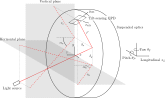
\includegraphics[width=0.7\linewidth]{figures/kagra_optical_lever_3d}
	\caption{Optical lever setup in KAGRA.}
	\label{fig:kagraopticallever3d}
\end{figure}

A 3D illustration of the optical lever setup is shown in Fig.~\ref{fig:kagraopticallever3d}.
For the current discussion, let's assume that the optical lever is well aligned so the beam spot miscentering at the optics $\delta_x$ and $\delta_y$ are zero.
Now, the lever arm of the optical lever can be an arbitrary vector, i.e. $\vec{r}=r_x\hat{x}+r_y\hat{y}+r_z\hat{z}$.
For the purpose of this discussion, let $\hat{x}$ be a direction aligned to the transverse direction of the main optics, $\hat{y}$ be a direction aligned to the vertical direction of the optics, and $\hat{z}$ be a direction aligned to the longitudinal direction of the optics.
Optical levers in KAGRA are aligned on a horizontal plane (i.e. $r_y=0$), or vertical plane (i.e. $r_x=0$).
But, let's assume that they are not zero.

If we project the beam onto a horizontal plane and a vertical plane (along the normal of the suspended optics), the beams have an incidence angle of $\alpha_h$ and $\alpha_v$ on the horizontal plane and the vertical plane, respectively.
It follows that the lever arm that amplifies the pitch angle is the length of the projection of the lever arm $\vec{r}$ on the vertical plane, $r_v$\footnote{Think of it as a cross-product $\vec{\theta}\times\vec{r}$. For example, for pitch, $-\theta_P\hat{x}\times\left(r_x\hat{x}+r_y\hat{y}+r_z\hat{z}\right) = \theta_P\left(-r_y\hat{z}+r_z\hat{y}\right)$, which is a displacement on the horizontal plane, and $r_v=\sqrt{r_y^2+r_z^2}$ is the corresponding lever arm that amplifies pitch.}.
Similarly, the lever arm amplifying the yaw angle is the length of the projection of the lever arm on the horizontal plane, $r_h$.
Therefore, a rotation in yaw $\theta_Y$ and pitch $\theta_P$ would cause the beam spot at the tip of the lever arm to shift by $\left(2r_h\right)\theta_Y$ and $\left(2r_v\right)\theta_P$, on the horizontal plane and vertical plane respectively.
Meanwhile, a longitudinal shift $x_L$ would cause the beam spot to shift by $\left(2\sin\alpha_h\right)x_L$ and $\left(2\sin\alpha_v\right)x_L$ on the horizontal plane and vertical plane, respectively.
From here, we can write the displacement of the beam spot as measured by the tilt-sensing QPD, placed at some distance $\vec{r}$ from the beam spot at the suspended optics plane.
The beam spot displacement is simply a superposition of that caused by a rotation and a longitudinal shift,
\begin{equation}
	x_\mathrm{tilt} = \left(2r_h\right)\theta_Y + \left(2\sin\alpha_h\right)x_L,
\end{equation}
and
\begin{equation}
	y_\mathrm{tilt} = \left(2r_v\right)\theta_P + \left(2\sin\alpha_v\right)x_L.
\end{equation}

Now, let's focus on the horizontal plane 



\subsection{Misalignment}


	\section{Measuring the sensing matrix}
	\bibliographystyle{plain}
	\bibliography{main_bib.bib}
\end{document}